\documentclass{standalone}

\usepackage{tikz}
\usetikzlibrary{arrows}
\usetikzlibrary{decorations.markings}
\usepackage{standalone}

\begin{document}

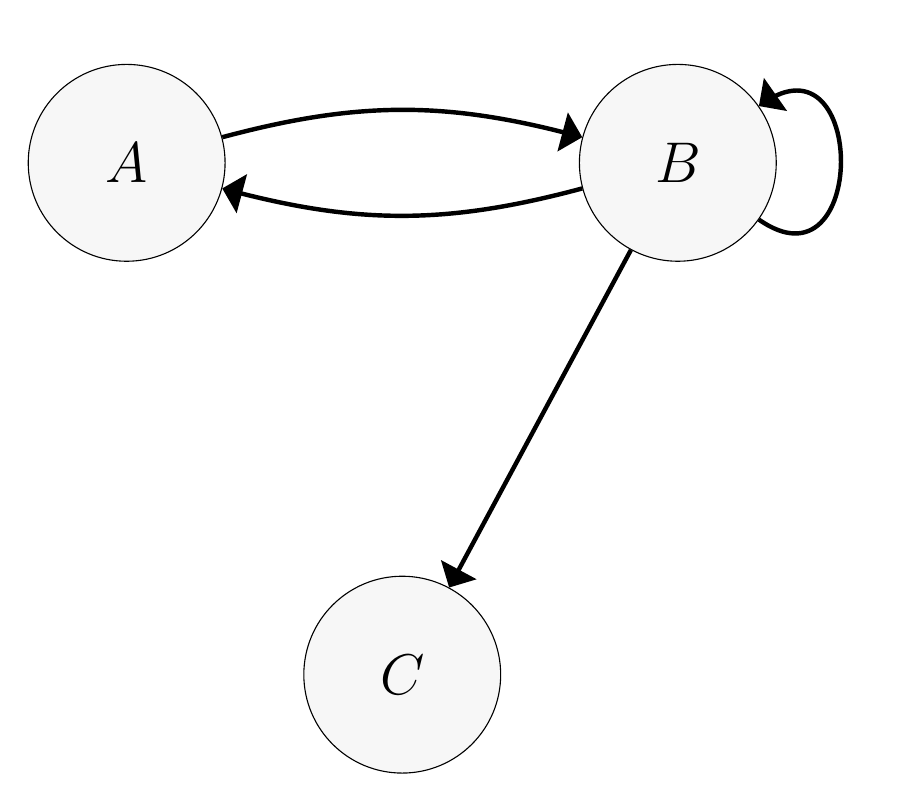
\begin{tikzpicture}

\node (A) [style={minimum size=2.5cm,draw=black,fill=black!3,text=black,shape=circle}] at (0, 13.5) {\huge{$A$}};
\node (B) [style={minimum size=2.5cm,draw=black,fill=black!3,text=black,shape=circle}] at (7, 13.5) {\huge{$B$}};
\node (C) [style={minimum size=2.5cm,draw=black,fill=black!3,text=black,shape=circle}] at (3.5, 7) {\huge{$C$}};

\draw[ultra thick, -triangle 90] (B) [bend left=15] to (A);
\draw[ultra thick, -triangle 90] (A) [bend left=15] to (B);
\draw[ultra thick, -triangle 90] (B) -- (C);
\draw[ultra thick, -triangle 90] (B) [out=-35, in=35, looseness=3] to (B);


\end{tikzpicture}

\end{document}